\documentclass[reqno]{amsart}

\usepackage{amsfonts,latexsym,amsthm,amssymb,amsmath,amscd,euscript,bm}
\usepackage[sc]{mathpazo}
\usepackage[margin = 2cm]{geometry}
\usepackage{enumitem}
\usepackage{hyperref}
% sets numbering of enumerate to a, b, c, ...
\renewcommand{\theenumi}{\alph{enumi}}

% Theorems, propositions, etc.
\newtheorem{theorem}{Theorem}
\newtheorem{proposition}[theorem]{Proposition}
\newtheorem{lemma}[theorem]{Lemma}
\newtheorem{corollary}[theorem]{Corollary}

\theoremstyle{definition}
\newtheorem{definition}[theorem]{Definition}
\newtheorem*{claim}{Claim}

\theoremstyle{remark}
\newtheorem*{remark}{Remark}
\newtheorem*{notation}{Notation}
\newtheorem*{example}{Example}

\usepackage{tikz-cd}

% Math blackboard font
\newcommand{\nc}{\newcommand}
\nc{\on}[1]{\operatorname{#1}}

\nc{\R}{\mathbb R}
\nc{\C}{\mathbb C}
\nc{\Q}{\mathbb Q}
\nc{\Z}{\mathbb Z}
\nc{\N}{\mathbb N}
\nc{\HH}{\mathbb H}
\nc{\DD}{\mathbb D}
\nc{\TT}{\mathbb T}
\nc{\EE}{\mathbb E}
\nc{\PP}{\mathbb P}

\nc{\cT}{\mathcal T}
\nc{\cA}{\mathcal A}
\nc{\cM}{\mathcal M}
\nc{\cR}{\mathcal R}
\nc{\cB}{\mathcal B}
\nc{\cG}{\mathcal G}
\nc{\cD}{\mathcal D}
\nc{\cS}{\mathcal S}
\nc{\cF}{\mathcal F}
\nc{\cL}{\mathcal L}
\nc{\cE}{\mathcal E}

\nc{\loc}{\text{loc}}

% Why the f*** would you ever use \epsilon
\renewcommand{\epsilon}{\varepsilon}
\renewcommand{\emph}{\textsc}
\renewcommand{\Re}{\operatorname{Re}}
\renewcommand{\Im}{\operatorname{Im}}

\let\vec\mathbf

\title
{
	\emph{Ordinary differential equations}
} 

\author{Jason Zhao}
\date{\today}

\begin{document}
\maketitle

\begin{abstract}
	We give an exposition of the initial data problem for ordinary differential equations, with a view towards non-linear evolutionary partial differential equations in mind. The material presented borrows a great deal from \cite[Chapter 1]{Tao2006}. 
\end{abstract}

\tableofcontents

\section{Preliminaries}
An \emph{ordinary differential equation} is an equation which governs the evolution of a function $u : I \to V$ mapping an interval $I \subseteq \R$ to a finite-dimensional vector space $V$ known as the \emph{state space}. Abstractly, they are equations which take the form 
	\begin{equation}
		G(u, \partial_t u, \dots, \partial_t^k u, t) = 0.
		\tag{nLin}
		\label{eq:nLin}
	\end{equation}	
for some given function $G : V^{k + 1} \times I \to W$, where $W$ is another finite-dimensional vector space. We are interested in the \emph{initial data problem}, also known as the Cauchy problem, in which we aim to find a $k$-times continuously differentiable solution satisfying \emph{initial data conditions},
	\begin{align*}
		u_{|t = 0}
			&= u_0, \\
		\partial_t u_{|t = 0}
			&= u_1,\\
			&\vdots \\
		\partial_t^{k - 1} u_{|t = 0}	
			&= u_{k - 1}	
	\end{align*}
for some $u_0, u_1, \dots, u_{k - 1} \in V$. 	

\subsection{Types of equations}

The most general form of an ODE is a fully \emph{non-linear} equation (\ref{eq:nLin}). This is a \emph{system of equations} when the codomain of $G$ has more than one dimension, otherwise it is a \emph{scalar equation}. If the number of equations $\dim W$ exceeds the degrees of freedom $\dim V$, then the equation is \emph{over-determined}, in which case one may require additional constraints on any initial data before a solution can be found. Conversely if there are fewer equations than degrees of freedom, the equation is \emph{under-determined}, and so there may be a multiplicity of solutions for any given data. 

We will only consider ODE which are \emph{fully determined}: the number of equations coincides with the degrees of freedom. In this case, assuming some non-degeneracy conditions, any non-linear ODE can be reduced to a \emph{quasi-linear} ODE, that is, one which is linear with respect to the highest-order derivatives. 

\begin{proposition}[Reduction to quasi-linear]
	Let $G : V^{k + 1} \times I \to V$ is continuously differentiable, and suppose that $u_k \mapsto G(u_0, u_1, \dots, u_{k - 1}, u_k, 0)$ is invertible. Then there exists there exists $F: V^{k + 1} \times I \to V$ such that
		\begin{equation}
			 \partial_t^{k + 1} u = F(u, \partial_t u, \dots, \partial_t^{k} u, t).\tag{qLin}\label{eq:qLin}
		\end{equation}	
\end{proposition}

\begin{proof}
	We differentiate the equation (\ref{eq:nLin}), obtaining by the chain rule
		\[ \partial_t G + \sum_{j = 0}^{k - 1} D_{u_j} G \cdot \partial_t^{j + 1} u + D_{u_k} G \cdot \partial_t^{k + 1} u = 0.\]
	Rearranging and inverting the matrix $D_{u_k} G$ gives the result. 	
\end{proof}


When the function $G$ in (\ref{eq:nLin}) does not depend on the time-variable $t$, we say the ODE is \emph{autonomous}, otherwise we say it is \emph{non-autonomous}. Autonomous ODEs enjoy the property of \textit{time-translation-invariance}, i.e. if $t \mapsto u(t)$ is a solution, then so is $t \mapsto u(t - t_0)$. Every non-autonomous system can be converted into an autonomous one by embedding the time-variable into the state-space. 

\begin{proposition}[Reduction to autonomy]
	Every non-autonomous ODE,
		\begin{align}
			G(u, \partial_t u, \dots, \partial_t^k u, t) 
			&= 0,\tag{nAut}\label{eq:nAut}
		\end{align}	
	can be reduced to an autonomous ODE,
		\begin{align}
			\widetilde G(\widetilde u, \partial_t \widetilde u, \dots, \partial_t^k \widetilde u)
			&= 0. \tag{Aut}\label{eq:Aut}
		\end{align}	
\end{proposition}

\begin{proof}
	Define $\widetilde u : I \to V \times I$ and $\widetilde G : (V \times I)^{k + 1} \times I \to W \times I$ by 
		\begin{align*}
			\widetilde u (t)
				&:= (u(t), t),\\
			\widetilde G((u_0, s_0), (u_1, s_1), \dots, (u_k, s_k))
				&:= (G(u_0, \dots, u_k), s_1 - 1).
		\end{align*}
	A routine check shows that every solution to (\ref{eq:nAut}) is a solution to (\ref{eq:Aut}), and conversely, every solution to (\ref{eq:Aut}) is a solution to (\ref{eq:nAut}) modulo time-translation. 
\end{proof}



\begin{example}
	The quasilinear non-autonomous ODE
		\[ \partial_t u = F(t, u) \]
	is equivalent to the \textit{system} of autonomous ODE
		\begin{align*}
			\partial_t u(t) 
				&= F(s, t), \\
			\partial_t s(t)
				&= 1. 	
		\end{align*}
\end{example}

The \emph{order} of an ODE refers to the order of the highest derivative occurring in the equation. Any $k$-th order system can be reduced to a first-order system at the cost of multiplying the degrees of freedom by $k$. 

\begin{proposition}[Reduction of order]
	Every $k$-th order quasi-linear ODE, 
		\begin{align}
			\partial_t^k  u
				&= F(u, \partial_t u, \dots \partial^{k - 1} u),
				\tag{$k^{\text{th}}$}
				\label{eq:kth}
		\end{align}
	can be reduced to a first-order quasi-linear ODE,
		\begin{align}
			\partial_t \widetilde u
				&= \widetilde F (u). 
				\tag{$1^{\text{st}}$}
				\label{eq:1st}
		\end{align}
\end{proposition}

\begin{proof}
	Set $\widetilde u : I \to V^k$ and $\widetilde F: V^k \to V^k$ to be
		\begin{align*}
			\widetilde u 
				&:= (u, \partial_t u, \dots, \partial_t^{k - 1} u) ,\\
			\widetilde F (u_0, \dots, u_{k - 1})
				&= (u_1, \dots, u_{k - 1}, F(u_0, \dots, u_{k - 1}))	.
		\end{align*}	
	Then $\widetilde u$ is a continuously differentiable solution to the first-order equation (\ref{eq:1st}) if and only if $u$ is $k$-times continuously differentiable solution to the $k$-th order equation (\ref{eq:kth}). 	
\end{proof}


\subsection{Notions of a solution}

With these reductions at hand, we focus our attention to the study of the initial data problem for first-order quasi-linear systems of equations on $\R^n$, 
\begin{equation}
	\begin{split}
		\partial_t u 	&= F(u), \\
		u_{|t = 0}		&= u_0.
	\end{split}\tag{IDP}	\label{eq:idp}
\end{equation}
If we assume the non-linearity is analytic, then one could hope to solve the ODE by differentiating the equation to obtain a recurrence relation for $\partial_t^k u$, and then show the corresponding formal power series for $u$ converges. Indeed, this is the approach of the Cauchy-Kowalevskaya theorem. However, without such strong assumptions on $F$, it is not clear how one could solve (\ref{eq:idp}) by ``classical'' (read: undergraduate calculus) methods. 

To get around this, often times it becomes easier to solve an equation by ``weakening'' the notion of a solution, giving access to tools from functional analysis when dealing with PDEs, or metric space topology in the case of ODEs. We say that a solution $u : [0, T] \to \R^n$ to (\ref{eq:idp}) is a
\begin{itemize}
	\item a \emph{classical solution} if $u \in C^1_\loc ([0, T])$ and satisfies the initial data problem for all $t \in [0, T]$ using the classical notion of the derivative. 
	
	\begin{figure}[h]
		\begin{center}
			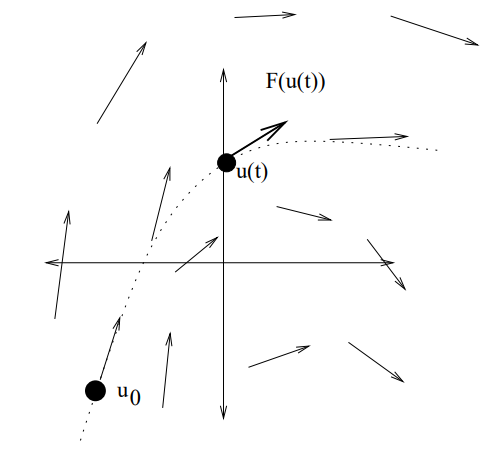
\includegraphics[scale = 0.5]{classical}
			\caption{The non-linearity $F(u)$ is regarded as a \textit{force} which governs the velocity $\partial_t u$ and thereby the evolution of the solution $u$.}
		\end{center}
	\end{figure}
	
	\item a \emph{strong solution} if $u \in C^0_\loc ([0, T])$ and solves the initial data problem in the integral sense that 
					\[ u(t) = u_0 + \int_0^t F(u(s))\, ds \]
				for all $t \in [0, T]$. 	
				
	\begin{figure}[h]
		\begin{center}
			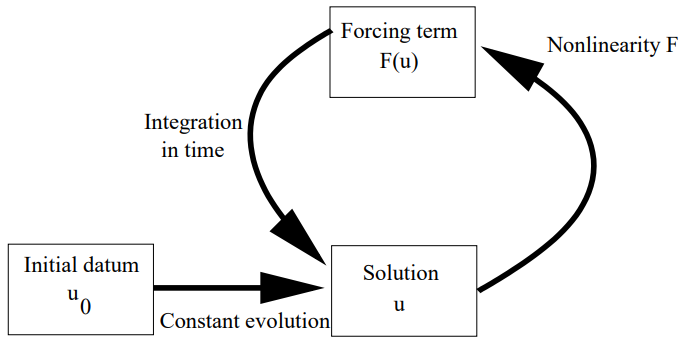
\includegraphics[scale = 0.5]{strong}
			\caption{The relationship between the solution $u$ and the non-linearity $F(u)$ can be viewed as a \textit{feedback loop} in which the solution influences the non-linearity, and vice versa.}
		\end{center}
	\end{figure}	
	
	\item a \emph{weak solution} if $u \in L^\infty ([0, T])$ which solves the initial data problem in the sense of distributions, i.e.
				\[ \int_0^T u(t) \psi (t) \, dt = u_0 \int_0^T \psi (t) \, dt + \int_0^T \psi (t) \left(\int_0^T F(u(s)) \, ds\right) dt \]
			for all test functions $\psi \in C_c^\infty ([0, T])$. 	
\end{itemize}

\begin{proposition}[Equivalence of notions]
	Let $F: \R^n \to \R^n$ be continuous and $u_0 \in \R^n$, then the notions of classical, strong, and weak solutions to the initial data problem (\ref{eq:idp}) are equivalent. 
\end{proposition}

\begin{proof}
	 It is clear that a classical solution is strong by the fundamental theorem of calculus, and that a strong solution is weak. If $u$ is a weak solution, we know that $t \mapsto F(u(t))$ is bounded and measurable and therefore
	\[ t \mapsto \int_0^t F(u(s)) \, ds \]
is Lipschitz continuous. Choose $\psi$ to be approximations to the identity concentrated at $t$, the weak formulation implies that
	\[ u(t) = u_0 + \int_0^t F(u(s)) \, ds \]
for a.e. $t$. It follow that $u$ is Lipschitz up to modification on a measure zero set, so it is a strong solution. Then $t \mapsto F(u(t))$ is in fact continuous, and so by the fundamental theorem of calculus $u \in C^1_\loc ([0, T])$ and solves the initial data problem classically. 
\end{proof}


\subsection{Well-posedness}

One should think of the initial data problem as governing the time evolution $\partial_t u$ of a physical state $u$ starting from an initial condition $u_0$. Not all ODEs are of physical relevance, though if it were to have one, and indeed these are the equations we care about, then we expect it to have the following properties:
	\begin{itemize}
		\item Existence: if a physical phenomenon is governed by an ODE, then it should correspond to a solution. 
		
		\item Uniqueness: physical reality is deterministic, the past determines the future, so there should only be one solution for each initial data. 
		
		\item Continuous dependence on initial data: the evolution of a physical phenomenon is stable under perturbations, so the solution should depend continuously on the initial data. 
	\end{itemize}
If the initial data problem (\ref{eq:idp}) satisfies these three criterion, then we say it is \emph{well-posed}. The concept of well-posedness was introduced by Hadamard in \cite{hadamard} as an attempt to clarify the link between differential equation and physics. 

For a more precise statement, we need to specify the space in which we look for solutions to the initial data problem, the time interval of existence, and the topology on the space of solutions. We say well-posedness is
	\begin{itemize}
		\item \emph{conditional} vs. \emph{unconditional} if well-posedness holds only in a subset $X \subseteq C^0 ([0, T] \to \R^n)$ vs. the entire space $X = C^0 ([0, T] \to \R^n)$, 
		
		\item \emph{local} vs \emph{global} if well-posedness holds only for finite time $[0, T]$ vs. infinite time $[0, \infty)$, 
		
		\item $C^{k, \alpha}$ if the solution map $u_0 \mapsto u$ is $C^{k, \alpha}$-differentiable, where differentiability is taken in a Frechet sense. 
	\end{itemize}
Our starting point will be to show local conditional $C^0$-well-posedness, which states that	for any $u_0^* \in \Omega$, there exists a time $T > 0$ and an open ball $B \subseteq \Omega$ containing $u_0^*$ and a subset $X \subseteq C^0([0, T] \to \R^n)$ such that for each $u_0 \in B$ there exists a unique strong solution $u \in X$, and furthermore the solution map $u_0 \mapsto u$ is continuous. 


\section{Existence}
\subsection{Analytic solutions}

Following our earlier remarks, we can formally differentiate the equation to obtain a recurrence relation for the derivatives of $u$. If one specifies initial data at $t = 0$, these relations fully determine all the derivatives $\partial_t^k u (0)$. In the case where the non-linearity is analytic, the formal power series for $u$ is the natural candidate for the solution to the initial data problem. 


\begin{theorem}[Cauchy-Kowalevskaya theorem]
	Let $F \in C^\omega (\R^n \to \R^n)$ be analytic, then there exists a unique analytic solution to the initial data problem (\ref{eq:idp}). 
\end{theorem}

\begin{proof}
	By replacing $u$ with $u - u_0$, it is not a loss of generality to prove solve the equation for initial data $u_0 = 0$. Our goal is to obtain an \textit{a priori} estimate on the growth of $\partial_t^m u(0)$ such that the \textit{ansatz}
		\[ u(t) := \sum_{n = 0}^\infty \frac{\partial^n_t u (0)}{m!} t^m \]	
	is shown to be analytic. It would follow by construction and the uniqueness theorem then that $\partial_t u - F(u) \equiv 0$ since the left-hand side is an analytic function which vanishes to every order at $t = 0$. Formally differentiating the equation, it follows from the chain rule and induction that the derivatives of $u$ can be written as a polynomial with non-negative coefficients in the derivatives of $F$ up to order $m - 1$,
		\[ \partial_t^m u = p_m ( F (u),  \nabla F(u), \dots, \nabla^{m - 1} F(u)) \]
	for some $p_m \in \N_0 [\vec x]$. Using the initial data $u(0) = 0$, it follows that $\partial_t^m u (0)$ are fully determined by $\nabla^j F(0)$ up to order $j < m$. Note that the polynomial $p_m$ is determined combinatorially, depending only on the order $m$. To estimate the growth of $\partial_t^m u (0)$, we argue by \textit{analytic majorisation}; non-negativity of the coefficients of $p_m$ imply 
		\begin{equation}
			|\partial^m_t u (0)| \leq \partial^m_t v(0)
			\tag{*}
			\label{eq:major}  
		\end{equation}	
	for any solution to the initial data problem	
		\begin{align*}
			\partial_t v 
				&= G(v) ,\\
			v_{|t = 0}
				&= 0,	
		\end{align*}
	for some analytic $G \in C^\omega (\R^n \to \R^n)$ such that $|\partial^m F_i (0)| \leq \partial^m G_i (0)$. Our strategy will be to choose $G$ such that the auxiliary ODE above is explicitly solvable for analytic $v$. The growth estimates on the power series of coefficients of $v$ also hold for those of $u$ via the majoristion (\ref{eq:major}), completing the proof. To construct $G$, we know from analyticity of $F$ that there exists $r > 0$ such that
		\[ |\nabla^m F(0)| \leq \frac{m!}{r^{m + 1}}. \]
	We construct $G$ such that the $m$-th order derivatives are precisely the right-hand side, namely
		\[  G_i (z_1, \dots, z_n) := \frac{1}{r - z_1 - \dots - z_n}. \]	
	For simplicity, consider the scalar case $n = 1$, the higher dimensional case is similar. By separation of variables, the explicit solution is given by $v(t) = r - r \sqrt{1 - 2t}$, which is clearly analytic in the region $|t| < r/2$. This completes the proof. 
\end{proof}


\subsection{Picard iteration}

	From the strong solution perspective, solving (\ref{eq:idp}) is equivalent to finding a \emph{fixed point} $\Phi_{u_0} (u) = u$ of the integral operator $\Phi_{u_0} : C^0 ([0, T] \to \R^n) \to C^0 ([0, T] \to \R^n)$ defined by 
		\[ (\Phi_{u_0} u)(t) := u_0 + \int_0^t F(u(s)) \, ds. \]
	We will argue by \textit{Picard iteration}. Schematically, we start off with an approximate solution $u_0$, and inductively construct subsequent approximates $u_{n}$ by inputting $u_{n - 1}$ into the integral operator,
		\[ u_n := \Phi_{u_0} (u_{n - 1}) = u_0 + \int_0^t F(u_{n - 1}(s)) \, ds .\]
	These approximate solutions are known as \emph{Picard iterates}, and the goal then is to show that this sequence $\{u_n\}_n$ converges uniformly to some $u$. If this were true, then by continuity of $\Phi_{u_0}$ and construction of the sequence, the limit $u$ would be a fixed point. A sufficient condition is if $\Phi_{u_0}$ is a \emph{contraction}, i.e. Lipschitz continuous with constant $L < 1$, 
	\[ || \Phi_{u_0} (u) - \Phi_{u_0} v||_{C^0[0, T]} \leq L ||u - v||_{C^0[0, T]}. \]
	\begin{figure}[h]
		\begin{center}
			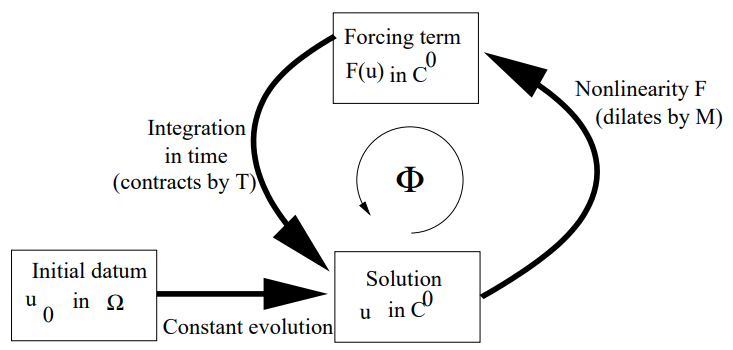
\includegraphics[scale = 0.6]{picard}
			\caption{The strong solution notion says that $u$ is determined by its past via integration in time. Thus for $T \ll 1$, the initial data $u_0$ is a good approximate solution. Iterating these approximations through the operator $\Phi_{u_0}$ converges provided we have some ``gain'' at each stage. }
		\end{center}
	\end{figure}
	
\begin{lemma}[Contraction mapping principle]
	Let $(X, d)$ be a complete non-empty metric space, and let $\Phi : X \to X$ be a contraction on $X$. Then there exists a unique fixed point $u = \Phi(u)$. Furthermore, if $u_0 \in X$ and we construct the sequence $\{u_n\}_n \subseteq X$ iteratively by 
		\[ u_{n + 1} := \Phi(u_n),\]
	then $u_n \to u$. 
\end{lemma}

\begin{proof}
	To show existence, we aim to show that the iterates $\{u_n\}_n$ form a Cauchy sequence. For $n, k \geq 0$, we obtain
		\begin{alignat*}{2}
			 d(u_n, u_{n + k}) 
			 	&= d(\Phi^n (u_0), \Phi^n (u_k))			
			 		&&\\
			 	&\leq c^n d(u_0, u_k) 
			 		&&\\
			 	&\leq c^n \left( d(u_0, \Phi(u_0)) + \dots + d(\Phi^{k - 1} (u_0), \Phi^k (u_0)) \right) 
			 		&&, \\
			 	&\leq 	c^n \sum_{j = 0}^{k - 1} c^j d(u_0, \Phi(u_0))
			 		&& \\
			 	&\leq \frac{c^n}{1 - c} d(u_0, \Phi(u_0))
			 		&&.	
		\end{alignat*}	 
	Since $0 < c < 1$, the above vanishes upon passing the limit $n \to \infty$, proving that the sequence is Cauchy. Since $X$ is complete, we know that there exists a limit $u \in X$. As contractions are continuous, 
		\[ \Phi(u) = \Phi( \lim_{n \to \infty} u_n) = \lim_{n \to \infty} \Phi(u_n) = \lim_{n \to \infty} u_{n + 1} = u.  \]
	To show uniqueness, suppose $v \in X$ is another fixed point, then by definition and the contraction inequality
		\[ d(u, v) \leq cd(u, v), \]	
	which, since $0 < c < 1$, can only hold if $d(u, v) = 0$ i.e. $u = v$. 
\end{proof}

\begin{theorem}[Picard-Lindelof existence theorem]
	Let $\Omega \subseteq \R^d$ be a domain, and suppose $F \in \dot C^{0, 1}_{\loc} (\Omega \to \R^d)$ is locally Lipschitz. For initial data $u_0 \in \Omega$ and $\epsilon \ll 1$, set
		\begin{align*}
			L
				&:= ||F||_{\dot C^{0, 1} (\overline{B_\epsilon (u_0)})} ,\\
			M
				&:= ||F||_{C^{0} (\overline{B_\epsilon (u_0)})}.	
		\end{align*}
	Then for $T < \min (\epsilon/M, 1/L)$, there exists a strong solution $u: [0, T] \to \overline{B_\epsilon (u_0)}$ to the initial data problem (\ref{eq:idp}). 
\end{theorem}

\begin{proof}
	The contraction mapping principle furnishes a solution provided we show that the integral operator $\Phi_{u_0}$ is a contraction mapping on the closed ball $C^0 ([0, T] \to \overline{B_\epsilon (u_0)})$. We first show $\Phi_{u_0}$ maps the desired space into itself: by choice of $T$ and $M$, we have 
		\begin{align*}
			 ||(\Phi_{u_0} u)(t) - u_0||_{C^0 [0, T]} 
			 	&\leq \int_0^T |F(u(s))| \, ds \leq TM \leq \epsilon. 
		\end{align*}
	Next, we show $\Phi_{u_0}$ is a contraction: 
		\[ ||\Phi_{u_0} u - \Phi_{u_0} v||_{C^0 [0, T]} \leq  \int_0^T |F(u(s)) - F(v(s))| \, ds \leq T L ||u - v||_{C^0}, \]
	where $TL < 1$ by construction. This completes the proof.
\end{proof}

\begin{remark}
	A common theme in solving ODEs and more generally PDEs is that we need to exploit some ``smallness'' to get an estimate or iteration to close. In this case, we exploit the time of existence $T$ to ``defeat'' any large oscillations from $F$ which could prevent the iteration from converging. 
\end{remark}


\subsection{Compactness solutions}

Suppose now we only had continuity of the non-linearity $F$ and no control over the Lipschitz norms. We again argue by approximation, this time approximating the equation and showing the corresponding solutions converge via \textit{compactness}, namely 

\begin{lemma}[Arzela-Ascoli theorem]
	Let $(X, d)$ be a compact metric space, and let $\cF \subseteq C(X)$ be a family of continuous functions. Then $\cF$ is pre-compact if and only if 
	\begin{itemize}
		\item $\cF$ is uniformly bounded, that is, $||f||_{C(X)} \lesssim 1$ uniformly in $f \in \cF$, 
		\item $\cF$ is equicontinuous, that is, for every $\epsilon > 0$ there exists a uniform $\delta > 0$ such that $|f(x) - f(y)| < \epsilon$ whenever $|x - y| < \delta$ for all $f \in \cF$.
	\end{itemize}
\end{lemma}

While we can approximate the non-linearity in the uniform topology by Lipschitz functions, there is no uniform control over the Lipschitz constants. Thus, following the proof of the Picard-Lindelof theorem, we cannot quantitatively show the approximate solutions exist on the same time interval existence. We instead turn to a more qualitative argument relying on \textit{continuous induction on time}. 

\begin{lemma}[Bootstrap argument]
	Let $f : [0, T) \to [0, \infty)$ be continuous, and suppose $f(0) \leq C$. Suppose that $f(t) \leq 2C$ implies the stronger bound $f(t) \leq C$, then the stronger bound holds for all time. 
\end{lemma}

\begin{proof}
	We argue by connectedness of the interval $[0, T)$. The set of times $A \subseteq [0, T)$ where $f(t) \leq 2C$ holds is
		\begin{itemize}
			\item non-empty, since $0 \in A$, 
			\item closed, since $f$ is continuous, 
			\item open, since if $t \in A$, then we in fact have the stronger bound $f(t) \leq C$, which by continuity allows us to propagate the weaker bound forward in time $f(t^+) \leq 2C$. 
		\end{itemize}
	Hence $A = [0, T)$. 
\end{proof}

\begin{remark}
	The weaker estimate $f(t) \leq 2C$ is known as a \emph{bootstrap assumption}. Since it in fact implies a stronger bound $f(t) \leq C$, the estimate ``picks itself up by its bootstraps''. 
\end{remark}

\begin{theorem}[Peano's existence theorem]
	Let $\Omega \subseteq \R^n$ be a domain and suppose $F \in C^0_{\loc} (\Omega \to \R^n)$ is continuous. Then for any $u_0 \in \Omega$, there exists a local solution to the initial data problem (\ref{eq:idp}).
\end{theorem}

\begin{proof}
	Assume without loss of generality $u_0 = 0$. There exists $\{ F_k \}_k \subseteq C^\infty (\Omega \to \R^n)$ such that $F_k \to F$ uniformly on compact sets. Smooth functions are locally Lipschitz, so, choosing a small closed ball $\overline{B_\epsilon (0)} \subseteq \Omega$, Picard-Lindelof furnishes local solutions $u_k : [0, T_k) \to B_\epsilon (0)$ to the initial data problems
	\begin{align*}
		\partial_t u_k 	
			&= F_k(u_k), \\
		{u_k}_{|t = 0}		
			&= 0
	\end{align*}
	We claim that there exists a uniform time interval $[0, T] \subseteq \bigcap_k [0, T_k)$ on which $\{u_k\}_k$ exist and are pre-compact. By uniform convergence, there exist uniform constant $M > 0$ such that $|F_k (u)| \leq M$ whenever $|u| \leq \epsilon$. Let $0 < T < \epsilon/(2M + 1)$, we make the bootstrap assumption that $|u_k| \leq \epsilon$ on the interval $[0, T]$. It follows that
		\[ |u_k (t)| \leq \int_0^T |F_k (u_k (s))| \, ds \leq T M \leq \frac\epsilon2 \]
	for all $t \in [0, T]$. The local well-posedness theory allows us to continue the solution, thus by continuous induction on time $u_k$ exists on $[0, \epsilon/(2M + 1)$ and satisfies the uniform bound $|u_k| \leq \epsilon$. Furthermore the equation implies $|\partial_t u_k| \leq M$. This proves $\{u_k\}_k$ is uniformly bounded and equicontinuous, so by Arzela-Ascoli we pass to a subsequence which converges uniformly to a continuous function $u$. As $F_k (u_k (t)) \to F(u(t))$ uniformly, we conclude $u$ is a desired strong solution, i.e. 
		\[ u(t) = \lim_{k \to \infty} u_k (t) = \lim_{k \to \infty} \int_0^t F_k (u_k (s)) \, ds = \int_0^t F (u(s)) \, ds\]
	for all $t \in [0, \epsilon/(2M + 1)]$. 	
\end{proof}


\begin{remark}
	Uniqueness may fail without further assumptions on the regularity of $F$; for example, letting $0 < \alpha < 1$, consider the initial data problem
			\begin{align*}
				\partial_t u 	&= |u|^\alpha, \\
				u_{|t = 0}		&= 0.
			\end{align*}
	Then 
		\[
			u_c (t) = 
				\begin{cases}
					0, 												&\text{if } x \leq c, \\
					(t - c)^\frac{1}{1 - \alpha}, 	&\text{if } t > c,
				\end{cases}
		\]		
	is an infinite family of solutions indexed by $c \geq 0$. Following the proof of Peano's existence theorem, we observe that uniqueness breaks down in that our solution depends on the choice of approximation by smooth functions. 
	
	\begin{figure}[h]
	\begin{center}
		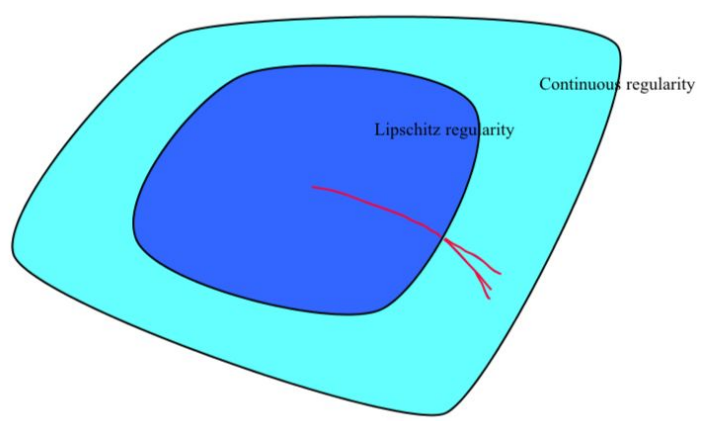
\includegraphics[scale = 0.5]{unique}
		\caption{Uniqueness fails once the solution leaves the regime of Lipschitz regularity. Approaching the boundary can be viewed as a \textit{blow-up criterion}, see Section 5 for details. }
	\end{center}
\end{figure}
\end{remark}

\section{Uniqueness}
As seen in Peano's theorem, uniqueness breaks down once the solution leaves the regime where the non-linearity is Lipschitz continuous. Thus we restrict our attention to solutions which stay within the state space $\Omega$. In this regime, we have uniqueness for $F \in \dot C^{0, 1}_{\loc} (\Omega \to \R^n)$, complementing the local existence theory. Our key ingredient will be Gronwall's inequality, which states that linear feedback bounds can at worst lead to exponential growth. 

\begin{lemma}[Gronwall's integral inequality]
	Let $u: [0, T] \to \R^+$ be a continuous and non-negative function, and suppose $u$ obeys the integral inequality
		\[ u(t) \leq A + \int_0^t B(s) u(s) \, ds \]
	for some $A \geq 0$ and $B :[0, T] \to \R^+$ continuous and non-negative. Then 
		\[ u(t) \leq A \exp \left( \int_0^t B(s) \,ds \right). \]	
	Moreover, this estimate is sharp, with equality when $u(t) := A \exp (\int_0^t B(s) \, ds)$. 	
\end{lemma}

\begin{proof}
	By a limiting argument we can assume $A > 0$. Differentiating the right-hand side of the integral inequality, the fundamental theorem of calculus and the inequality imply
		\[ \frac{d}{dt} \left(A + \int_0^t B(s) u(s) \, ds \right) \leq B(t) \left( A + \int_0^t B(s) u(s) \, ds \right) .\]
	Hence by the chain rule
		\[ \frac{d}{dt} \log \left(  A + \int_0^t B(s) u(s) \, ds  \right) \leq B(t). \]	
	Integrating, we obtain
		\[  \log \left(  A + \int_0^t B(s) u(s) \, ds  \right) \leq \log A + \int_0^t B(s) \, ds, \]
	which upon exponentiating completes the proof. 		
\end{proof}

\begin{theorem}[Picard-Lindelof uniqueness theorem]
	Let $\Omega \subseteq \R^n$ be a domain, and suppose $F \in \dot C^{0, 1}_{\loc} (\Omega \to \R^n)$ is locally Lipschitz. If $u, v \in C^1_{\loc} ([0, T] \to \Omega)$ are solutions to the initial data problem (\ref{eq:idp}), then $u \equiv v$. 
\end{theorem}

\begin{proof}
	Since $[0, T]$ is a compact interval, $u$ and $v$ range over a compact subset of $\Omega$. Therefore by local Lipschitz continuity there exists $L > 0$ such that $|F(u) - F(v)| \leq L |u - v|$. The difference of the two solutions satisfy
		\[ \partial_t (u - v) = F(u) - F(v).\]
	Integrating and applying the triangle inequality gives 
		\[ |u(t) - v(t)| \leq \int_0^t |F(u(s)) - F(v(s))| \, ds \leq L \int_0^t |u(s) - v(s)| \, ds .\]
	We conclude from Gronwall's inequality that $u \equiv v$. 	
\end{proof}

\section{Continuous dependence on initial data}
Studying the proof of the Picard-Lindelof existence theorem, we see that the corresponding solutions to initial data in any domain $\Omega \subseteq \R^n$ can be taken to exist on the same time-interval $[0, T]$, provided there exists a uniform bound and Lipschitz constant on an $\epsilon$-neighborhood $\overline{B_\epsilon (\Omega)} \subseteq \R^n$. Combined with uniqueness, the \emph{solution operator} $S : \Omega \to C^0 ([0, T] \to \R^n)$ mapping initial data to solutions is well-defined. Our goal in this section will be to study the regularity of this operator. 



\subsection{$C^{0, 1}$-dependence}

We begin with Lipschitz dependence on initial data. This is a simple consequence of retracing the proof of the Picard-Lindelof theorem and tracking down the constants. 

\begin{theorem}[$C^{0, 1}$-dependence on data]
	Let $\Omega \subseteq \R^n$ be a domain, and suppose $F \in C^{0, 1}(\overline{B_\epsilon (\Omega)} \to \R^n)$ is Lipschitz and bounded with constants
		\begin{align*}
			L &:= ||F||_{\dot C^{0, 1} (\overline{B_\epsilon (\Omega)})}, \\
			M &:= ||F||_{C^{0} (\overline{B_\epsilon (\Omega)})}.
		\end{align*}
	Then for $T< \min (\epsilon/M, 1/L)$, the solution operator $S : \Omega \to C^0 ([0, T] \to \R^n)$	 is well-defined and Lipschitz continuous with constant $\frac{1}{1 - TL}$.
\end{theorem}

\begin{proof}
	The solution $S u_0$ is a fixed point of $\Phi_{u_0}$, so we can write
		\[ S u_0 - Sv_0 = \Phi_{u_0} (S u_0) - \Phi_{v_0} (S v_0) + u_0 - v_0. \]
	Following the Picard-Lindelof existence proof, we showed that the integral operators $\Phi_{u_0}$ are contractions on $C^0([0, T] \to \Omega)$ for every initial data $u_0 \in \Omega$ with Lipschitz constant $TL$. Thus, taking norms above and applying the triangle inequality, we obtain 
		\[ || Su_0 - Sv_0||_{C^0 [0, T]} \leq ||\Phi_{u_0} (Su_0) - \Phi(S v_0)||_{C^0 [0, T]} + |u_0 - v_0| \leq  TL || Su_0 - Sv_0||_{C^0 [0, T]} + |u_0 - v_0|.\]
	Rearranging, 
		\[ || Su_0 - Sv_0||_{C^0 [0, T]} \leq \frac{1}{1 - TL} |u_0 - v_0|,  \]
	as desired. 		
\end{proof}

\subsection{$C^1$-dependence}

Assume the non-linearity is continuously differentiable, we want to show that the solution operator is continuously differentiable. This is meant in the \textit{Frechet} sense, i.e. there exists a linear operator $DS(u_0) : \R^n \to C^0 ([0, T] \to \R^n)$ such that 
	\[ \lim_{v \to 0}\left|\left| \frac{S(u_0 + v) - S(u_0) - DS(u_0)}{|v|} \right|\right|_{C^0[0, T]} = 0 \]
and $u_0 \to DS(u_0)$ is continuous. As in the finite-dimensional codomain setting, this is equivalent to the existence and continuity of ``partial'' Frechet derivatives, so we will consider smooth one-parameter families of initial data $h \mapsto u_0 (h)$ for $|h| \ll 1$, and show that the solution $u(t, h) := Su_0 (h) (t)$ is continuously differentiable in $h$. The total derivative $DS$ can be reconstructed from the partial derivatives $\partial_h u$.

 The difference quotient in $h$ satisfies 
	\[ \partial_t \left( \frac{u(t, h) - u(t, 0)}{h} \right) = \frac{F(u(t, h)) - F(u (t, h_0))}{h},  \]
then, assuming $u$ is continuously differentiable in $h$ and $F$ is continuously differentiable, taking $h \to 0$ gives
	\[ \partial_t \partial_h u (t, 0) = \nabla F(u(t, 0)) \cdot \partial_h u (t, 0). \]
This shows that $\partial_h u$, if it exists, satisfies the \emph{linearised equation},
	\begin{equation}
		\begin{split}
			\partial_t A 
		 	&= \nabla F (u) \cdot A,\\
		 A_{|t = 0}
		 	&= \partial_h u_0 (0)	.
		\end{split}
		\tag{Lin}
		\label{eq:linear}
		\end{equation}
\textit{A priori}, we do not know if $u$ is continuously differentiable with respect to its initial data, so we instead work backwards by studying the linearised initial data problem. Heuristically, the \textit{dynamics} of the original equation are dominated by the linearised equation, as the higher-order terms in the non-linearity are negligible. 


\begin{theorem}[$C^{1}$-dependence on data]
	Let $\Omega \subseteq \R^n$ be a domain, and suppose $F \in C^{1}(\overline{B_\epsilon (\Omega)} \to \R^n)$ is continuously differentiable and bounded with constants
		\begin{align*}
			L &:= ||F||_{\dot C^{1} (\overline{B_\epsilon (\Omega)})}, \\
			M &:= ||F||_{C^{0} (\overline{B_\epsilon (\Omega)})}.
		\end{align*}
	Then for $T< \min (\epsilon/M, 1/L)$, there exists a unique solution $u \in C^2_{\loc} ([0, T] \to \R^n)$ to (\ref{eq:idp}), and the solution operator $S : \Omega \to C^0 ([0, T] \to \R^n)$	 is well-defined and continuously differentiable.
\end{theorem}

\begin{proof}
	Using the equation and the chain rule, we see that the solution obtained from Picard-Lindelof iteration has regularity $u \in C^2_{\loc} ([0, T] \to \R^n)$. By local well-posedness, the linearised equation (\ref{eq:linear}) admits a solution in $[0, T]$. We claim that $\partial_h u(t, 0)$ exists and $A = \partial_h u (t, 0)$. Translating, this argument shows that $\partial_h u (t, h)$ exists for all $t \in [0, T]$ and $|h| \ll 1$. Set
		\[ B(t) := \frac{u(t, h) - u(t, 0)}{h} - A(t) , \]
	our goal is to show that $B (t) \to 0$ as $h \to 0$ for each fixed $t$. Differentiating and using the equations, 
		\begin{align*}
			\partial_t B (t)
				&= \frac{F(u(t, h)) - F(u(t, 0))}{h} - \nabla F(u(t, 0)) \cdot A(t)  \\
				&=  \int_0^1 \frac{u(t, h) - u(t, 0)}{h} \cdot \nabla F(s \cdot u(t, h) + (1 - s) \cdot u (t, 0)) \, ds - \nabla F(u(t, 0)) \cdot A(t) \\
				&= C_1 (t) \cdot B(t) + C_2 (t) \cdot A(t),
		\end{align*}	
	where
		\begin{align*}
			C_1 (t) 
				&:=\int_0^1 \nabla F(s \cdot u(t, h) + (1 - s) \cdot u (t, 0)) \, ds, \\
			C_2 (t)
				&:= \int_0^1  \left(\nabla F(s\cdot u(t, h) + (1 - s)\cdot u (t, 0)) - \nabla F (u(t, 0))\right)\, ds .
		\end{align*}	
	From our regularity assumptions, we see that $|A|, |C_1|, |C_2| \leq N$ for some uniform constant $N \gg 1$. Thus, integrating the expression for $\partial_t B$ and applying the bounds above, we obtain 
		\[ |B(t)| \leq |B(0)| + TN ||C_2||_{C^0[0, T]}  + N \int_0^t |B(s)| \, ds.  \]	
	Using Gronwall's inequality, this implies
		\[ |B(t)| \leq e^{t} \left( |B(0)| + TN ||C_2||_{C^0[0, T]} \right)  \]	
	Since $h \mapsto u(0, h)$ and $F$ are continuously differentiable, $|B(0)|$ and $||C_2||_{C^0[0, T]}$ vanish as $h \to 0$. We conclude from construction of $B$ that $\partial_h u$ exists and is given by $A$. 
	
	It remains to show that $\partial_h u$ is continuous in $h$ uniformly in $t$. Again, by translation it is not a loss of generality to show the result for $h = 0$. Integrating the linearised equation, we obtain
		\begin{align*}
			|\partial_h u (t, h) - \partial_h u (t, 0)|
				&\leq |\partial_h u(0, h) - \partial_h u (0, 0)| + \int_0^t |\nabla F (u(s, h)) \cdot \partial_h u (s, h) - \nabla F(u(s, 0)) \cdot \partial_h u(s, 0)| \, ds\\
				&\leq |\partial_h u(0, h) - \partial_h u (0, 0)| + \int_0^t |\nabla F (u(s, h)) - \nabla F(u(s, 0))|  \cdot |\partial_h u(s, h)| \, ds \\
				&\qquad+ \int_0^t |\nabla F(u(s, 0)) \cdot | \partial_h u(s, h) - \partial_h u(s, 0)| \, ds
		\end{align*}
	By Gronwall's inequality.
		\[ |\partial_h u (t, h) - \partial_h u (t, 0)| \leq e^{L t} \left( |\partial_h u_0 (h) - \partial_h u_0 (0)| + C \int_0^t   |\nabla F (u(s, h)) - \nabla F(u(s, 0))| \, ds \right) \]	
	for some $L, C > 0$. Since $\partial_h u_0$ and $\nabla F$ are continuous, the right-hand side vanishes uniformly in $t$ as $h \to 0$. 	
\end{proof}

\begin{corollary}[$C^{k}$-dependence on data]
	Let $\Omega \subseteq \R^n$ be a domain, and suppose $F \in C^{k}(\overline{B_\epsilon (\Omega)} \to \R^n)$ is continuously differentiable and bounded with constants
		\begin{align*}
			L &:= ||F||_{C^{k} (\overline{B_\epsilon (\Omega)})}, \\
			M &:= ||F||_{C^{0} (\overline{B_\epsilon (\Omega)})}.
		\end{align*}
	Then for $T< \min (\epsilon/M, 1/L)$, the solution operator $S : \Omega \to C^0 ([0, T] \to \R^n)$	 is well-defined and continuously differentiable.
\end{corollary}

\begin{proof}
	Induction on $k$ and the $C^1$-wellposedness theory. 
\end{proof}

\section{Maximal solutions}
In the previous sections, we have studied the \textit{local} well-posedness theory of the initial data problem. Inductively applying the local theory to the end-time of existence for any solution $u$, we can show that there exists a \emph{maximal time of existence} $T_{\text{max}}$, i.e. there does not exist a solution $v : [0, T^+] \to \R^n$ to (\ref{eq:idp}) such that $u \equiv v$ on $[0, T_{\text{max}})$. We refer to the solution defined on $[0, T_{\text{max}})$ as the \emph{maximal solution}. 

\begin{theorem}[Continuation criterion]
	Let $\Omega \subseteq \R^n$ be a domain, and suppose $F \in \dot C^{0, 1}_{\loc} (\Omega \to \R^n)$ is locally Lipschitz. If $u : [0, T] \to \Omega$ is a solution to the initial data problem (\ref{eq:idp}) which does not approach the boundary of $\Omega$ or blow-up, i.e.
		\begin{align*}
			\lim_{t \to T}\operatorname{dist} (u(t), \partial \Omega) 
				> 0, \qquad \text{and} \qquad
			\lim_{t \to T} |u(t)| 
				< \infty,
		\end{align*}
	then $u$ can be extended to a solution on $[0, T^+]$. 
\end{theorem}

\begin{proof}
	Since $u$ does not approach the boundary or blow-up, there exists a closed ball $\overline{B_\epsilon(u(T))} \subseteq \Omega$ on which we can continue the solution via the local theory. 
\end{proof}

\begin{corollary}[Existence of maximal solutions]
	Let $\Omega \subseteq \R^n$ be a domain, and suppose $F \in \dot C^{0, 1}_{\loc} (\Omega \to \R^n)$ is locally Lipschitz. Then there exists a maximal solution defined on a half-open interval $[0, T_{\text{max}})$. 
\end{corollary}

\begin{proof}
	The maximal time interval of existence must be half-open, since if $u$ is defined on $[0, T]$, then by local well-posedness it can be extended to $[0, T^+]$. Define the maximal time interval of existence $[0, T_{\text{max}})$ as the union of all intervals $[0, T]$ for which one has a solution to the initial data problem (\ref{eq:idp}). By the uniqueness theorem, we may glue these solutions together to obtain a maximal solution.
\end{proof}

\begin{corollary}[Blow-up criterion]
	Let $\Omega \subseteq \R^n$ be a domain, and suppose $F \in \dot C^{0, 1}_{\loc} (\Omega \to \R^n)$ is locally Lipschitz. If $u$ is a maximal solution to the initial data problem (\ref{eq:idp}) and $T_{\text{max}} < \infty$, then either
		\begin{align*}
			\lim_{t \to T_{\text{max}}}\operatorname{dist} (u(t), \partial \Omega) 
				= 0, \qquad \text{or} \qquad
			\lim_{t \to T_{\text{max}}} |u(t)| 
				= \infty.
		\end{align*}
\end{corollary}

\begin{proof}
	Suppose $u$ does not blow-up, then there exists a compact subset $K \subseteq \Omega$ on which $u(t) \in K$ for all $[0, T_{\text{max}})$, and denote
		\begin{align*}
			L
				&:= ||F||_{\dot C^{0, 1} (\overline{B_\epsilon(K)})} ,\\
			M
				&:= ||F||_{C^{0}(\overline{B_\epsilon(K)})}.
		\end{align*}	
	Then for all $t$, local well-posedness theory allows us to extend $u$ to a solution on $[t, t + T]$ for $T < \min (\epsilon/M, 1/L)$. Taking $t \uparrow T_{\text{max}}$ contradicts maximality of $T_{\text{max}}$. 
\end{proof}

\begin{remark}
	The proposition does not apply to global solutions, e.g. the constant function $u \equiv u_0$ is a global solution to $u' = 0$ and $u(0) = u_0$, and it does not exhibit blow-up. 
\end{remark}

\begin{example}
	Consider the initial data problem
	\begin{align*}
		\partial_t u	
			&= u^2, \\
		u_{|t = 0}	
			&= u_0.
	\end{align*}
The map $u \mapsto u^2$ is locally Lipschitz, however the solution
	\[ u(t) = \frac{1}{1/u_0 - t} \]	
admits blow-up in finite time, namely $t = 1/u_0$. Following the proof of Picard-Lindelof, we see that the length of time in which a solution exists depends inversely with the local Lipschitz constant, and so the blow-up in this case coincides with the blow-up of the local Lipschitz constant of $u \mapsto u^2$. 
\end{example}

This example suggests that if we had uniform control over the Lipschitz constant, then we could obtain a global solution, which are obviously maximal. 

\begin{proposition}[Existence of a global solution]
	Let $\Omega \subseteq \R^n$ be a domain, and suppose $F \in C^{0, 1} (\Omega \to \R^n)$ is Lipschitz continuous, then there exists a unique global solution to the initial data problem  (\ref{eq:idp}).
\end{proposition}

\begin{proof}
	Denote
		\[ L := ||F||_{\dot C^{0, 1} (\Omega)} \]
	and let $0 < T < 1/L$. It follows that the integral operator $\Phi_{u_0}$ as defined in the proof of the Picard-Lindelof existence theorem is a contraction on the space $C^0([0, T] \to \Omega)$, 
		\[ ||\Phi_{u_0}u  - \Phi_{u_0} v||_{C^0[0, T]}\leq  \int_0^T |F(u(s)) - F(v(s))| \, ds \leq TL ||u - v||_{C^0[0, T]}. \]
	The contraction mapping principle furnishes a unique solution $u : [0, T] \to \Omega$ to the initial data problem. We iterate the Picard-Lindelof scheme at each endpoint of the previous construction, supposing we had a solution $u_k : [0, kT] \to \Omega$ to the initial data problem for some $k \in \N$, and solving 
		\begin{align*}
			u_{k + 1}' (t) &= F(u_{k + 1} (t)), \\
			u_{k + 1} (kT)	&= u_k (kT).
		\end{align*}
	By Picard-Lindelof iteration, we obtain a solution $u_{k + 1} : [0, (k + 1) T] \to \Omega$ satisfying the original problem. Proceeding inductively in $k$ furnishes a global solution $u: [0, \infty) \to \Omega$.
\end{proof}


\bibliographystyle{alpha}
\bibliography{biblio}


\end{document}